\subsection{The completion of a Zariski ring}

PROPOSITION 9. Let A be a commutative Noetherian ring and m an ideal of A; let A be given the m-adic topology. For \(\hat{\mathbf{A}}\) to be a faithfully flat A-module, it is necessary and sufficient that A be a Zariski ring.

For every finitely generated A-module M, the canonical mapping \(M \to M \otimes_{A} \hat{A}\) is identified with the canonical mapping \(M \to \hat{M}\) from M to its Hausdorff completion with respect to the m-adic topology (no. 4, Theorem 3) and the kernel of this mapping is then the closure of \(\{0\}\) in M with respect to this topology. As we already know that \(\hat{A}\) is a flat A-module (no. 4, Theorem 3), the proposition follows from the characterization of faithfully flat modules (Chapter I, §3, no. 1, Proposition 1 (b)) and the characterization of Zariski rings (no. 3, Proposition 6).

If A is a Zariski ring and E is a finitely generated A-module, we may (by virtue of Proposition 9) identify E with a subset of \(\hat{E}\) by means of the canonical mapping \(j_{E}: E \to \hat{E}\) . With this identification:

COROLLARY 1. Let A be a Zariski ring, E a finitely generated A-module and F a submodule of E. Then \(\mathbf{F} = \hat{\mathbf{F}} \cap \mathbf{E} = (\hat{\mathbf{A}}\mathbf{F}) \cap \mathbf{E}\) .

This is a special case of Chapter I, § 3, no. 5, Proposition 10 (ii) and it also follows from no. 3, Proposition 6.

COROLLARY 2. Let A be a Zariski ring and E a finitely generated A-module. If \(\hat{\mathbf{E}}\) is a free \(\hat{\mathbf{A}}\) -module, E is a free A-module.

Let \(\mathfrak{m}\) be a defining ideal of \(\mathbf{A}\) , which is therefore contained in the Jacobson radical of \(\mathbf{A}\) . We apply the criterion of Chapter II, § 3, no. 5, Proposition 5: the canonical mapping \(j_{\mathrm{E}}: \mathrm{E} \to \hat{\mathrm{E}}\) defines a bijection \(i_{\mathrm{E}}: \mathrm{E} / \mathfrak{m}\mathrm{E} \to \hat{\mathrm{E}} / (\mathfrak{m}\mathrm{E})^{\wedge}\) ; similarly the canonical mapping \(j_{\mathrm{A}}: \mathrm{A} \to \hat{\mathrm{A}}\) defines a bijection \(i_{\mathrm{A}}: \mathrm{A} / \mathfrak{m} \to \hat{\mathrm{A}} / \hat{\mathfrak{m}}\) , which is a ring isomorphism. Then \((\mathfrak{m}\mathrm{E})^{\wedge} = \hat{\mathrm{A}}. \mathfrak{m}\mathrm{E} = \hat{\mathfrak{m}}\hat{\mathrm{E}}\) (no. 4, Theorem 3), so that \(\hat{\mathrm{E}} / (\mathfrak{m}\mathrm{E})^{\wedge}\) is given an \((\hat{\mathrm{A}} / \hat{\mathfrak{m}})\) -module structure and hence (by means of \(i_{\mathrm{A}}\) ) an \((\mathrm{A} / \mathfrak{m})\) -module structure. It is immediate that \(i_{\mathrm{E}}\) is \((\mathrm{A} / \mathfrak{m})\) -linear, so that it is an \((\mathrm{A} / \mathfrak{m})\) -module isomorphism. As \(\hat{\mathrm{E}} / \hat{\mathfrak{m}}\hat{\mathrm{E}}\) is a free \((\hat{\mathrm{A}} / \hat{\mathfrak{m}})\) -module, \(\mathrm{E} / \mathfrak{m}\mathrm{E}\) is a free \((\mathrm{A} / \mathfrak{m})\) -module.

On the other hand, let \(v: \mathfrak{m} \otimes_{\mathbf{A}} \mathbf{E} \to \mathbf{E}\) be the canonical homomorphism; as \((\mathfrak{m} \otimes_{\mathbf{A}} \mathbf{E}) \otimes_{\mathbf{A}} \hat{\mathbf{A}}\) is canonically identified with \(\hat{\mathfrak{m}} \otimes_{\mathbf{A}} \hat{\mathbf{E}}\) and \(\mathbf{E} \otimes_{\mathbf{A}} \hat{\mathbf{A}}\) with \(\hat{\mathbf{E}}\) (no. 4, Theorem 3), the hypothesis that \(\hat{\mathbf{E}}\) is a free \(\hat{\mathbf{A}}\) -module implies that the homomorphism \(v \otimes 1: \hat{\mathfrak{m}} \otimes_{\hat{\mathbf{A}}} \hat{\mathbf{E}} \to \hat{\mathbf{E}}\) is injective. As \(\hat{\mathbf{A}}\) is a faithfully flat A-module (Proposition 9), we conclude that \(v\) is injective (Chapter I, § 3, no. 1, Proposition 2) and the conditions for applying the above mentioned criterion are indeed fulfilled.

COROLLARY 3. Let A be a Zariski ring such that \(\hat{\mathbf{A}}\) is an integral domain and let \(\mathfrak{a}\) be an ideal of A. If the ideal \(\mathfrak{a}\hat{\mathbf{A}}\) of \(\hat{\mathbf{A}}\) is principal, \(\mathfrak{a}\) is principal. This is a special case of Corollary 2.

COROLLARY 4. Let A be a Zariski ring such that \(\hat{\mathbf{A}}\) is an integral domain, L the field of fractions of \(\hat{\mathbf{A}}\) and \(\mathbf{K} \subset \mathbf{L}\) the field of fractions of A; then \(\hat{\mathbf{A}} \cap \mathbf{K} = \mathbf{A}\) .

Clearly \(\mathbf{A} \subset \hat{\mathbf{A}} \cap \mathbf{K}\) ; on the other hand, if \(x \in \hat{\mathbf{A}} \cap \mathbf{K}\) , then \(\hat{\mathbf{A}}x \subset \hat{\mathbf{A}}\) and hence, as \(\hat{\mathbf{A}}x = \hat{\mathbf{A}} \otimes_{\mathbf{A}} (\mathbf{A}x)\) (no. 4, Theorem 3), \(\hat{\mathbf{A}} \otimes_{\mathbf{A}} ((\mathbf{A}x + \mathbf{A}) / \mathbf{A}) = 0\) . As \(\hat{\mathbf{A}}\) is a faithfully flat A-module (Proposition 9), we deduce that \(\mathbf{A}x \subset \mathbf{A}\) , whence \(x \in \mathbf{A}\) .

COROLLARY 5. Let A be a commutative Noetherian ring, E, F two finitely generated A-modules and u: E → F an A-homomorphism. For every maximal ideal m of A, let A(m) (resp. E(m), F(m)) denote the Hausdorff completion of A (resp. E, F) with respect to the m-adic topology and u(m): E(m) → F(m) the corresponding homomorphism to u. For u to be injective (resp. surjective, bijective, zero), it is necessary and sufficient that u(m) be so for every maximal ideal m of A.

We know that for \(u\) to be injective (resp. surjective, bijective, zero), it is necessary and sufficient that \(u_{\mathfrak{m}}: \mathrm{E}_{\mathfrak{m}} \to \mathrm{F}_{\mathfrak{m}}\) be so for every maximal ideal \(\mathfrak{m}\) of \(\mathbf{A}\) (Chapter II, § 3, no. 3, Theorem 1). We now note that \(\mathbf{A}_{\mathfrak{m}}\) is a Noetherian local ring (Chapter II, § 2, no. 4, Corollary 2 to Proposition 10) and hence a Zariski ring and there is a canonical A-algebra isomorphism \(\hat{\mathbf{A}}_{\mathfrak{m}} \to \mathbf{A}(\mathfrak{m})\) (§ 2, no. 13, Proposition 18). On the other hand (beginning of no. 4), there is a commutative diagram

\[
\begin{array}{l} \mathrm{E} _ {\mathfrak {m}} \otimes_ {\mathbf {A} _ {\mathfrak {m}}} \mathrm{A} (\mathfrak {m}) \longrightarrow \mathrm{E} \otimes_ {\mathbf {A}} \mathrm{A} (\mathfrak {m}) \longrightarrow \mathrm{E} (\mathfrak {m}) \\ u _ {\mathfrak {m}} \otimes 1 \Biggl \downarrow \qquad \qquad \qquad \qquad \Biggl \downarrow u \otimes 1 \qquad \qquad \Biggl \downarrow u (\mathfrak {m}) \\ \mathrm{F} _ {\mathfrak {m}} \otimes_ {\mathbf {A} _ {\mathfrak {m}}} \mathrm{A} (\mathfrak {m}) \longrightarrow \mathrm{F} \otimes_ {\mathbf {A}} \mathrm{A} (\mathfrak {m}) \longrightarrow \mathrm{F} (\mathfrak {m}) \end{array}
\]

where the horizontal arrows on the left arise from the associativity of the tensor product and the isomorphisms \(E_{m} \rightarrow E \otimes_{A} A_{m}\) , \(F_{m} \rightarrow F \otimes_{A} A_{m}\) ; as E and F are finitely generated A-modules, it follows from no. 4, Theorem 3 that the rows of this diagram consist of isomorphisms; thus we are reduced to proving that \(u_{m}\) being injective (resp. surjective, bijective, zero) is equivalent to \(u_{m} \otimes 1\) being so. But this follows from the fact that \(\hat{A}_{m}\) (and hence also \(A(m)\) ) is a faithfully flat \(A_{m}\) -module by Proposition 9 (Chapter I, § 3, no. 1, Propositions 1 and 2).

PROPOSITION 10. Let A, B be two Zariski rings, \(\hat{A}\) , \(\hat{B}\) their completions, \(f\colon A\to B\) a continuous ring homomorphism and \(\hat{f}\colon\hat{A}\to\hat{B}\) the homomorphism obtained from \(f\) by passing to the completions; if \(\hat{f}\) is bijective, the A-module B is faithfully flat.

As A and B are Hausdorff, the hypothesis that \(\hat{f}\) is bijective implies first that \(f\) is injective. Identifying (algebraically) A with \(f(A)\) by means of \(f\) and \(\hat{A}\) with \(\hat{B}\) by means of \(\hat{f}\) , we then obtain the inclusions \(A \subset B \subset \hat{A} = \hat{B}\) ; we know that \(\hat{A}\) is a faithfully flat A-module and a faithfully flat B-module (Proposition 9); we conclude that B is a faithfully flat A-module (Chapter I, § 3, no. 4, Remark 2).

PROPOSITION 11. Let A be a Noetherian local ring, m its maximal ideal, \(\hat{\mathbf{A}}\) its m-adic completion and B a ring such that \(\mathbf{A} \subset \mathbf{B} \subset \hat{\mathbf{A}}\) . Suppose that B is a Noetherian local ring whose maximal ideal n satisfies the relation \(n = mB\) . Then

\[
\mathfrak {n} ^ {k} = \mathfrak {m} ^ {k} \mathrm{B} = \hat {\mathfrak {m}} ^ {k} \cap \mathrm{B}
\]

for all \(k \geqslant 1\) , the \(\mathfrak{n}\) -adic topology on \(\mathbf{B}\) is induced by the \(\hat{\mathfrak{m}}\) -adic topology on \(\hat{\mathbf{A}}\) , \(\mathbf{B}\) is a faithfully flat \(\mathbf{A}\) -module and there is an isomorphism of \(\hat{\mathbf{A}}\) onto the \(\mathfrak{n}\) -adic completion \(\hat{\mathbf{B}}\) of \(\mathbf{B}\) , which extends the canonical injection \(\mathbf{A} \to \mathbf{B}\) .

It is sufficient to verify the relation \(n^{k} = \hat{m}^{k} \cap B\) , for, as B is dense in \(\hat{A}\) and the n-adic topology is induced by the \(\hat{m}\) -adic topology, the last assertion will follow from General Topology, Chapter II, §3, no. 9, Corollary 1 to Proposition 18 and the last but one from Proposition 10. The injection \(j_{A}: A \to \hat{A}\) (resp. \(j_{B}: B \to \hat{A}\) ) defines by taking quotients an injective homomorphism

\[
i _ {\mathbf {A}} \colon \mathrm{A} / (\hat {\mathfrak {m}} \cap \mathrm{A}) \rightarrow \hat {\mathrm{A}} / \hat {\mathfrak {m}}
\]

(resp. \(i_{B}\) : B/(m ∩ B) → Â/m). We know that m ∩ A = m and that \(i_{A}\) is bijective, hence \(i_{B}\) is bijective, which shows that B/(m ∩ B) is a field, hence that m ∩ B is a maximal ideal of B and therefore m ∩ B = n.~As \(\hat{A} = A + \hat{m}\) , \(B = A + n = A + mB\) ; by induction on k we deduce that

\[
\mathbf {B} = \mathbf {A} + \mathfrak {m} ^ {k} \mathbf {B} = \mathbf {A} + \mathfrak {n} ^ {k}
\]

for all \(k > 1\) . As \(\mathfrak{n}^k \subset \hat{\mathfrak{m}}^k \cap \mathbf{B}\) , it is sufficient to show that \(\hat{\mathfrak{m}}^k \cap \mathbf{B} \subset \mathfrak{n}^k\) ; if \(b \in \hat{\mathfrak{m}}^k \cap \mathbf{B}\) , we may write \(b = a + z\) where \(a \in \mathbf{A}\) , \(z \in \mathfrak{n}^k\) ; whence

\[
a = b - z \in \hat {\mathfrak {m}} ^ {k} \cap \mathrm{A} = \mathfrak {m} ^ {k} \subset \mathfrak {n} ^ {k}
\]

and \(b \in \mathfrak{n}^k\) .

* An important case where this applies is the following: B is the ring of integral series in n variables over a complete valued field, which converge in the neighbourhood of 0, A is the local ring

\[
\mathrm{K} [ \mathrm{X} _ {1}, \dots , \mathrm{X} _ {n} ] _ {\mathfrak {p}}
\]

where p is the maximal ideal consisting of the polynomials with no constant term and \(\hat{A}\) is the ring of formal power series \(K[[X_{1},\ldots,X_{n}]]\) . *

\pandocbounded{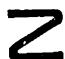
\includegraphics[keepaspectratio]{images/part002_72a4a9a7.jpg}}

Remark. A local ring B such that \(A \subset B \subset \hat{A}\) , whose maximal ideal n is equal to mB and whose n-adic topology is induced by the m-adic topology on \(\hat{A}\) , is not necessarily Noetherian (Exercise 14).

PROPOSITION 12. Let A be a commutative Noetherian ring, m an ideal of A, S the multiplicative subset \(1 + m\) of A and E a finitely generated A-module. Under these conditions:

\begin{enumerate}
\def\labelenumi{(\roman{enumi})}
\item
  \(\mathbf{S}^{-1}\mathbf{A}\) is a Zariski ring with the \((\mathbf{S}^{-1}\mathfrak{m})\) -adic topology.
\item
  The canonical mapping \(f \colon \mathbf{E} \to \mathbf{S}^{-1}\mathbf{E}\) is continuous if \(\mathbf{E}\) is given the \(\mathfrak{m}\) -adic topology and \(\mathbf{S}^{-1}\mathbf{E}\) the \((\mathbf{S}^{-1}\mathfrak{m})\) -adic topology and \(\hat{f} \colon \hat{\mathbf{E}} \to (\mathbf{S}^{-1}\mathbf{E})^{\wedge}\) is an isomorphism.
\end{enumerate}

Every element of \(1 + (\mathbf{S}^{-1}\mathfrak{m})\) is of the form

\[
1 + (m / \left(1 + m ^ {\prime}\right)) = (1 + m + m ^ {\prime}) / (1 + m)
\]

where \(m \in m\) and \(m' \in m\) ; it is therefore invertible in \(S^{-1}A\) , which proves that \(S^{-1}m\) is contained in the Jacobson radical of \(S^{-1}A\) ; as \(S^{-1}A\) is Noetherian (Chapter II, §2, no. 4, Corollary 2 to Proposition 10), \(S^{-1}A\) is a Zariski ring with the \((\mathrm{S}^{-1}\mathrm{m})\) -adic topology, which proves (i). Let us show (ii). For all n \textgreater{} 0,

\[
\bar {f} ^ {- 1} ((S ^ {- 1} m) ^ {n} E) = \bar {f} ^ {- 1} (S ^ {- 1} (m ^ {n} E)) = m ^ {n} E:
\]

for clearly first of all \(f(\mathfrak{m}^n\mathrm{E}) \subset \mathrm{S}^{-1}\mathfrak{m}^n\mathrm{E}\) ; conversely, let \(x\) be an element of \(f^{-1}(\mathrm{S}^{-1}\mathfrak{m}^n\mathrm{E})\) ; then there exist elements \(m', m''\) of \(\mathfrak{m}\) and \(x'' \in \mathfrak{m}^n\mathrm{E}\) such that \((1 + m')((1 + m'')x - x'') = 0\) , whence \((1 - m)x = x'\) , where

\[
m = - \left(m ^ {\prime} + m ^ {\prime \prime} + m ^ {\prime} m ^ {\prime \prime}\right) \in \mathfrak {m}
\]

and \(x' = (1 + m')x'' \in \mathfrak{m}^n\mathrm{E}\) ; we conclude that

\[
x = (1 + m + \dots + m ^ {n - 1}) x ^ {\prime} + m ^ {n} x \in \mathfrak {m} ^ {n} \mathrm{E}.
\]

This proves that \(f\) is a strict morphism. Moreover, the kernel of \(f\) , which is the set of \(x \in \mathbf{E}\) for which there exists some \(s \in \mathbf{S}\) such that \(sx = 0\) , is identical with the kernel of the canonical mapping \(j: \mathbf{E} \to \hat{\mathbf{E}}\) (no. 2, Proposition 5). Then there is a topological isomorphism \(f_0: j(\mathbf{E}) \to f(\mathbf{E})\) such that \(f = f_0 \circ j\) ; as \(j\) is a topological isomorphism, the problem reduces to verifying that \(f(\mathbf{E})\) is dense in \(\mathbf{S}^{-1}\mathbf{E}\) . Now every element of \(\mathbf{S}^{-1}\mathbf{E}\) may be written as \(x / (1 - m)\) , where \(m \in \mathfrak{m}\) , and it is immediately verified that

\[
x / (1 - m) \equiv ((1 + m + \dots + m ^ {n - 1}) x) / 1 (\mathrm{mod.} \mathrm{S} ^ {- 1} \mathrm{m} ^ {n} \mathrm{E})
\]

which completes the proof.

